\chapter{Tutoriel}
\label{chap:tutoriel}

    % ============ Prise en main de l'ARDrone ===============
    \section{Prise en main de l'ARDrone}
    \label{sec:prise_en_main_de_l_ardrone}
        L'ARDrone est un quadricoptère grand public contrôlable en wifi avec un smartphone. Dans le cadre du PAO, nous avons pour objectif de le faire voler en asservissant sa position dans l'espace grâce au système OptiTrack.

        % ---------------- Test de vol ----------------
        \subsection{Test de vol}
            Avant de s'aventurer à commander le drone depuis un PC, nous avons désiré savoir s'il était fonctionnel. Pour cela nous avons téléchargé l'application \footnote{\url{https://itunes.apple.com/fr/app/free-flight/id373065271?mt=8} et \url{https://play.google.com/store/apps/details?id=com.parrot.freeflight&hl=fr}} fournie par Parrot (la marque du drone), dont la figure~\ref{fig:application_ardrone} donne un aperçu.

            \begin{figure}[h]
              \centering
              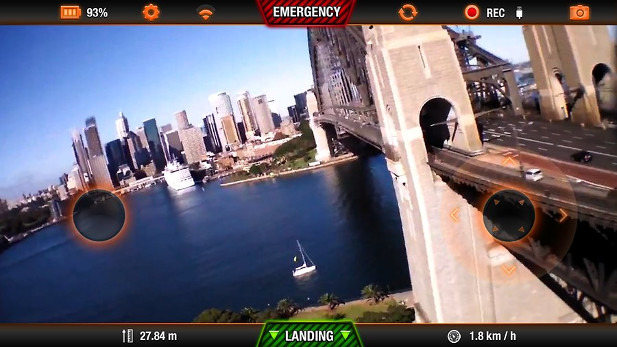
\includegraphics[height=8cm]{images/application_ardrone.jpg}
              \caption{Application pour ARDrone}
              \label{fig:application_ardrone}
            \end{figure}

            Une fois la batterie installée à bord, le drone s'allume tout seul et diffuse un réseau wifi dont le SSID ressemble à \textit{ardrone\_XXXX}. Il faut alors connecter le smartphone au réseau wifi du drone et lancer l'application téléchargée. \\

            Le drone est simple à piloter, le bouton \textit{take off} fait s'envoler le drone en mode stationnaire à 1 mètre d'altitude. Les sticks présents à l'écran permettent de l'incliner dans la direction souhaitée, de modifier son altitude, et de changer son orientation. Le bouton \textit{land} permet de le faire atterrir. Si le vol d'essai s'est déroulé sans problème, le drone est alors fonctionnel.


    % ============ Prise en main du système OptiTrack ===============
    \section{Prise en main du système OptiTrack}
    \label{sec:prise_en_main_du_systeme_optitrack}
        % ---------- Prérequis --------------
        \subsection{Prérequis}
            Pour pouvoir à la fois se connecter au serveur du logiciel Motive et au drone, il faut tout d'abord connecter l'ordinateur sur le réseau du drone. Pour cela, brancher la batterie au drone. Le drone s'allume tout seul et diffuse un réseau wifi dont le SSID ressemble à \textit{ardrone\_XXXX}. Ensuite seulement, démarrer le logiciel Motive. La figure~\ref{fig:motive} donne un aperçu de l'interface du logiciel Motive.

            \begin{figure}[h]
              \centering
              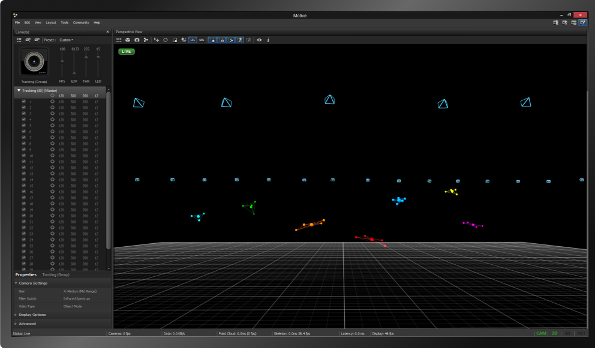
\includegraphics[height=10cm]{images/motive.png}
              \caption{Logiciel Motive}
              \label{fig:motive}
            \end{figure}

        % ---------- Calibration des caméras et de l'origine --------------
        \subsection{Calibration des caméras et de l'origine}
            Brancher la clé d'activation USB à l'ordinateur (celle-ci est la licence de Motive). Ensuite, brancher les caméras au hub USB, le hub sur le secteur et à l'ordinateur. À l'ouverture du logiciel, choisir \emph{perform camera calibration}, puis cliquer sur \emph{start wanding} en haut à droite. Cliquer sur \emph{continue} si un warning s'affiche. Prendre l'objet qui ressemble à un râteau avec 3 petites boules au bout, puis faire de grands mouvements de balancier dans la pièce jusqu'à ce que la précision passe en ``very-high''. Appuyer sur \emph{calculate} (le calcul de calibration prend environ 5 secondes). Le lien suivant \footnote{\url{https://www.youtube.com/watch?v=cNZaFEghTBU}} redirige vers la vidéo officielle d'Optitrack pour calibrer les caméras. \\

            Une fois la calibration des caméras effectuée, il faut paramétrer l'origine de l'espace 3D. Pour cela, placer le ``L'' (le repère) à l'origine voulue dans la pièce (nous avons choisi l'axe Z orienté vers le tableau). Cette position aura comme valeur (0, 0, 0) dans Motive. Sélectionner les 3 points du ``L'' et cliquer sur \emph{set ground plane} en haut à droite. Sauvegarder la calibration au besoin (nous conseillons de refaire la calibration à chaque utilisation du système si les caméras ne sont pas fixées définitivement).

        % ---------- Création d'un rigidbody --------------
        \subsection{Création d'un rigidbody}
            Une fois la calibration effectuée, il faut créer un rigidbody du drone pour pouvoir détecter sa position en temps réel. Pour cela, cliquer sur la rubrique \emph{layout} dans le menu de la barre du haut. Puis \emph{create}. Vous pouvez maintenant enlever le ``L'' pour positionner le drone à l'origine. Sélectionner les marqueurs constituant le drone et cliquer sur \emph{create from selection}. Le lien suivant \footnote{\url{https://www.youtube.com/watch?v=iMPh7JhlCqc&index=4&list=PLdKrdVGpQ5OZSlQDCyYFT-iOo1Qmfzl7Z}} redirige vers la vidéo officielle d'Optitrack pour créer des ``rigidbodies'' et mettre des labels sur les marqueurs.

        % ---------- Lancement du serveur --------------
        \subsection{Lancement du serveur}
            Pour lancer le serveur, sélectionner \emph{view} dans la barre de menu et cliquer sur \emph{data streaming}. Ensuite, cocher la case \emph{broadcast frame data}. Le mot ``NET'' en bas à droite devient orange.



